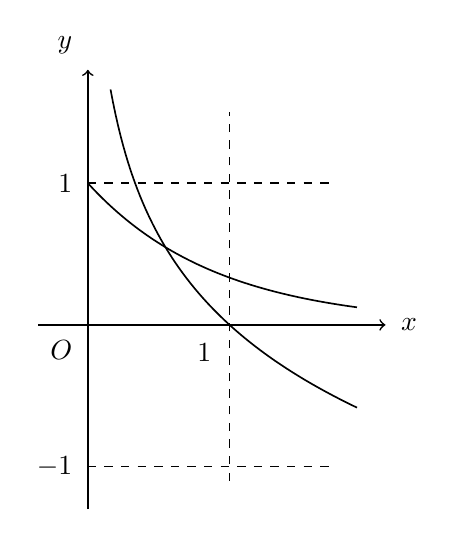
\begin{tikzpicture}[x=1.8cm,y=1.8cm,line width=.6pt,font=\normalsize]
\draw[->] (-.35,0)--(2.1,0) node[right=2pt] {$x$};
\draw[->] (0,-1.3)--(0,1.8) node[above left=2pt] {$y$};
\node[below left=2pt] at (0,0) {$O$};
\draw[dashed] (0,1)--(1.75,1);\draw[dashed] (0,-1)--(1.75,-1);\draw[dashed] (1,-1.1)--(1,1.5);
\node[left=2pt] at (0,1) {$1$};\node[left=2pt] at (0,-1) {$-1$};\node[below left=3pt] at (1,0) {$1$};
\draw[domain=0:1.9,samples=100] plot (\x,{pow(1/3,\x)});
\draw[domain=.16:1.9,samples=100] plot (\x,{ln(\x)/ln(1/3)});
\end{tikzpicture}
